\documentclass{article}
\usepackage{geometry}
\geometry{paperwidth=21cm,
paperheight=29.7cm,
margin=1cm}
\usepackage{amsmath}
\usepackage{mathfmv}
\usepackage{siunitx}
\usepackage{pgf}
\usepackage{tikz}
\usepackage{pgfplots}
\pgfplotsset{compat=1.18}
\begin{document}
\[
H(p)=0.1111111111111111\dfrac{p^2}{0.3p^2+1p+1}
\]
\begin{center}
\begin{tikzpicture}[trim axis left]
\begin{axis}[ticklabel style = {font=\normalsize},
width=0.9\textwidth,
height=0.25\textheight,
grid=both,
major grid style={black!40},
label style={font=\large},
xmode=log,ymode=normal,
xlabel={},
ylabel={Gain (\si{\decibel})},
xtick={0.1,1.0,10.0,100.0},
ytick={-40,-32,-24,-16,-8,0,8,16,24,32,40},
xticklabels={$10^{-1}$,$10^{0}$,$10^{1}$,$10^{2}$},
yticklabels={-40,-32,-24,-16,-8,0,8,16,24,32,40},
xmin=0.1,xmax=100.0,
ymin=-40,ymax=40]
\addplot[ultra thick, blue,domain=0.1:100.0,samples=256]{-9.54242509439325+40*log10(x)-10*log10(9.0+(x+(0.0))*(x+(0.0)))-10*log10(1.0+(x+(0.0))*(x+(0.0)))};
\addplot[line width=2pt,red,dashed,domain=0.1:1.0, samples=16]{-19.084850188786497+40*log10(x)};
\addplot[line width=2pt,red,dashed,domain=1.0:3.0, samples=16]{-19.084850188786497+40*log10(x)+(-20.0)*log10(x/1.0)};
\addplot[line width=2pt,red,dashed,domain=3.0:100.0, samples=16]{-19.084850188786497+40*log10(x)+(-20.0)*log10(x/1.0)+(-20.0)*log10(x/3.0)};
\end{axis}
\end{tikzpicture}

\begin{tikzpicture}[trim axis left]
\begin{axis}[ticklabel style = {font=\normalsize},
width=0.9\textwidth,
height=0.25\textheight,
grid=both,
major grid style={black!40},
label style={font=\large},
xmode=log,ymode=normal,
xlabel={Pulsation (\si{\radian\per\second})},
ylabel={Phase (\si{degree})},
xtick={0.1,1.0,10.0,100.0},
ytick={-180,-171,-162,-153,-144,-135,-126,-117,-108,-99,-90},
xticklabels={$10^{-1}$,$10^{0}$,$10^{1}$,$10^{2}$},
yticklabels={-180,-171,-162,-153,-144,-135,-126,-117,-108,-99,-90},
xmin=0.1,xmax=100.0,
ymin=-180,ymax=-90]
\addplot[ultra thick, blue,domain=0.1:100.0,samples=256]{180+(-1)*atan2(x/1.0,1)+(-1)*atan2(x/3.0,1)};
\addplot[line width=2pt,red,dashed,domain=0.1:1.0,samples=16]{180};
\draw[line width=2pt,red,dashed](axis cs:1.0,180) -- (axis cs:1.0,90.0);
\addplot[line width=2pt,red,dashed,domain=1.0:3.0,samples=16]{90.0};
\draw[line width=2pt,red,dashed](axis cs:3.0,90.0) -- (axis cs:3.0,0.0);
\addplot[line width=2pt,red,dashed,domain=3.0:100.0,samples=16]{0.0};
\end{axis}
\end{tikzpicture}
\end{center}
\paragraph{Fonctions réelles du gain et du déphasage}
\[
G(\omega)=|H(\jw)|=\dfrac{0\left(- \omega^{2}\right)}{- \frac{\omega^{2}}{3} + \frac{4 j \omega}{3} + 1}
\]
\[
G_{dB}(\omega)=-9+40\log\omega-10\log{\left(1+\left(\frac{\omega}{\omega_1}\right)^2\right)}-10\log{\left(1+\left(\frac{\omega}{\omega_2}\right)^2\right)}
\]
\[
\phi(\omega)=\arg{H(\jw)}=180-\arctan{\left(\frac{\omega}{\omega_1}\right)}-\arctan{\left(\frac{\omega}{\omega_2}\right)}
\]
\paragraph{Quelques valeurs particulières calculées}
\begin{center}
\begin{tabular}{ccc}
\hline
$\omega$ (\si{\radian\per\second}) & Gain (\si{\decibel}) & Phase (\si{\degree})\\
\hline
     0.10000 &    -59.13289 &    172.38025\\
\hline
     0.19953 &    -47.27358 &    164.91112\\
\hline
     0.39811 &    -35.79959 &    150.73303\\
\hline
     0.79433 &    -25.50355 &    126.70867\\
\hline
\textbf{     1.00000} & \textbf{   -22.55273} & \textbf{   116.56505}\\
\hline
     1.58489 &    -17.60930 &     94.40279\\
\hline
\textbf{     3.00000} & \textbf{   -13.01030} & \textbf{    63.43495}\\
\hline
     3.16228 &    -12.74389 &     61.03992\\
\hline
     6.30957 &    -10.53532 &     34.43545\\
\hline
    12.58925 &     -9.80961 &     17.94515\\
\hline
    25.11886 &     -9.61081 &      9.09048\\
\hline
    50.11872 &     -9.55969 &      4.56857\\
\hline
   100.00000 &     -9.54677 &      2.29130\\
\hline
\end{tabular}
\end{center}
\end{document}
